\documentclass[12pt,fleqn]{article}
\setlength{\parindent}{0pt}
\usepackage{graphicx}
\usepackage{listings}
\usepackage[latin5]{inputenc}
\setlength{\parskip}{8pt}
\setlength{\parsep}{0pt}
\setlength{\headsep}{0pt}
\setlength{\topskip}{0pt}
\setlength{\topmargin}{0pt}
\setlength{\topsep}{0pt}
\setlength{\partopsep}{0pt}
\setlength{\mathindent}{0cm}

\begin{document}
MIT OCW Cok Degiskenli Calculus - Ders 13

Lagrange Carpanlari (Multipliers)

Amac $f(x,y,z)$ gibi birden fazla degisken iceren bir fonksiyonu maksimize
etmek, degisik olan, $x,y,z$ degiskenlerinin birbirinden bagimsiz
ol\textbf{ma}masi. Bu degiskenlerin arasindaki iliski $g(x,y,z)=c$ gibi bir
fonksiyon tarafindan gosteriliyor olabilir, $c$ bir sabittir. Yani
$f(x,y,z)$'i minimize ya da maksimize ediyoruz ve bunu sadece $g(x,y,z)=c$
sartina / sinirlama ifadesine (constraint) uyan $x,y,z$ degerleri icin yapiyoruz.

Bunun icin hangi teknigi kullaniriz? Yollardan biri, eger sinirlama ifadesi
basit ise, belki bir degiskeni cebirsel olarak cozebiliriz (digerleri
baglaminda ifade ederek), sonra geri $f$'e sokariz, boylece klasik bir min
/ maks problemi elde ederiz, ki o tur bir problemi cozmeyi artik biliyoruz.

Fakat bazen $x,y,z$ degiskenleri icin analitik cozum mumkun olmaz, o zaman
farkli teknikler kullanmamiz gerekir. Bu derste ogrenecegimiz teknikler
bunlar olacak. 

Uygulama baglaminda, Lagrange Carpanlari bize niye ilgilendiriyor? Belki
fizik, termodinamik dersinde gormussunuzdur, sicaklik, hacim ve basinc
degerleri vardir, ve bu degerler birbirinden bagimsiz
degildir. Termodinamikte $pv = nrt$ denklemi vardir, gerci burada analitik
olarak basitlestirme yapabilirdik, ama bazi sartlarda tum degiskenleri
oldugu gibi tutmayi isteyebiliriz. 

Simdiye kadar min / maks problemleri icin gordugumuz kritik nokta bulma
tekniklerinin burada ise yarayamacagini hemen belirtelim. O kritik noktalar
$g(x,y,z)=c$ sinirlama ifadesini tatmin etmiyor olabilirler. Baska bir seye
ihtiyacimiz var. 

Ornek

Hiperbol $xy =3$ uzerinde olan ve orijine en yakin noktayi bul. 

Aslinda bu soruyu temel geometri kullanarak cozebiliriz, fakat burada
Lagrange Carpanlari kullanarak cozecegiz, cunku iyi bir ornek. 

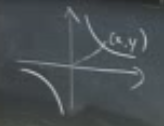
\includegraphics[height=2cm]{13_1.png}

Neyi minimize edelim? Mesela $f(x,y) = \sqrt{x^2 + y^2}$ olur mu? Olabilir,
ama karekok ifadesinden kurtulursak daha iyi olur. 

O zaman

\[ min \ f(x,y) = x^2 + y^2 \]

\[ ki, \ xy = 3  \]

Yani sinirlama ifadesi $g(x,y) = xy$ olarak sectik. 

Grafige bakalim. Yuvarlaklar $f(x,y)$ konturlari, yesil okla gosterilen
mesela $f(x,y) = 20$ konturu. Bu kontur ust sag kose ve sol alt kosede
gosterilen hiperbolu kesiyor mu? Evet. Fakat $f(x,y) = 10$, vs. diyerek
daha kucuk yuvarlaklar elde edebilir miyim? Evet. Fakat bir noktadan sonra
bu halkalar hiperbolu kesmeyecektir. 

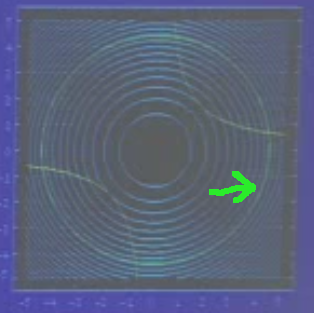
\includegraphics[height=4cm]{13_2.png}

Aradigimiz $x,y$ degerleri hiperbole teget olan, olabilecek en kucuk
yuvarlak.

Cozum icin tegetlik kavramindan faydalanabiliriz. Eger olabilecek en
minimal $f$, her iki fonksiyonun kesit egrilerinin teget oldugu noktada
ise, bu noktayi bulmaya ugrasabilirim. 

Iki kesit egrisi birbirine teget ise, onlarin teget duzlemi paraleldir,
eger oyleyse, bu duzlemlerin normalleri birbirine paralel olmalidir. 

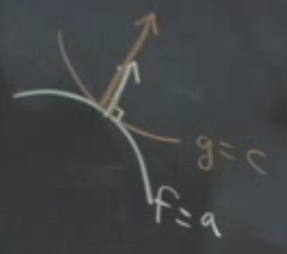
\includegraphics[height=4cm]{13_3.png}

Bu normallerin ayni boyda olmasi gerekmez, yukaridaki gibi, ama paralel
olmalari gerekir. 


\end{document}
